% !Mode:: "TeX:UTF-8"

\chapter{引言}

\pagenumbering{arabic}
\setcounter{page}{1}
在工业场景下,动态系统建模在过程控制、状态估计、系统预测等众多领域都起到了举足轻重的支撑作用。由于现实世界大部分的动态系统具有非线性、高扰动、强耦合等复杂特性,从机理角度建模系统动态过程的传统分析方法难以满足实际应用要求。伴随着工业监测技术的不断完善以及生产自动化、信息化水平的不断提升,各种大型设备及生产过程均安装了用于实时监测数据的传感器。 
由于监测数据获取成本低廉,且近年来大数据挖掘、机器学习等基础理论及技术日趋完善,
使得基于深度学习的复杂工业系统建模方法广受学者们的关注。然而,系统建模问题本身的高复杂性以及被辨识系统的多样性使得不同模型结构与训练方法在辨识精度以及训练效率方面具有极大的差异。
如何根据目标系统的不同特性,设计合理的参数化模型并有效地适配系统的先验属性,以获得最佳的建模效果,是复杂工业系统建模、智能优化控制等领域内亟待解决的关键问题。本文分别面向具有\textbf{长时延非线性、周期多阶段性、随机非确定性}的三种复杂工业系统,提出了以常微分方程网络为骨架的三种模型架构,\textbf{有效实现了以系统先验为指导、以离线数据为原料、以神经网络为骨架,端到端建模复杂动态系统的目标}。
同时,
本文在识别模型的基础上,\textbf{提出了基于有模型强化学习的复杂工业系统在线控制优化方法},并成功应用于工业实践,
成功实现了深度学习技术在真实工业系统建模与决策场景下的落地。
\section{研究背景与意义}
    
% 当前,新一轮科技革命和产业变革加速发展,新一代信息技术正在与工业生产 深度融合,自动化、信息化、智能化已经成为全球工业制造发展的重要方向。
% 2020年李克强总理发布的《政府工作报告》中,明确提出“推动制造业升级”、“推进智能制造”的要求。如何工业生产利用智能化技术,将,

% 为了实现工业4.0、工业互联网、数字孪生等伟大技术愿景,其中


% 复杂工业系统的控制与优化是典型的交叉学科,计算机、自动化、控制工程、仪器仪表等。
% 伴随着人工智能与数据科学的发展,数据驱动的复杂系统建模与控制优化技术逐渐应用。
% 现存问题:如何合理地将深度学习与工业过程特性深度融合,同时有效地指导系统优化并实现智能控制,对此部分的研究迫在眉睫。
% 本文面向具有长时延特性、周期多阶段性、非确定性的三类复杂工业系统,提出一套基于ODE-Net的动态系统建模方法,并在构建模型的基础上,提出了基于有模型强化学习理论的控制优化方法,并成功应用于工业实践。实现了xxx目标,为数据驱动的工业系统建模及控制优化提供了新的研究思路。

% \subsection{动态系统辨识及有模型控制的起源与发展}

% 基于数据驱动的复杂工业系统预测建模方法可以分成两大类:离散时间(Discrete Time, DT)系统建模和连续时间系统建模。

%%%%% 注释 %%%%%%%%
复杂工业系统及设备的分析与优化技术涉及了集工业制造、自动控制、计算机、人工智能等多学科知识,长久以来受到了国内外学者的广泛关注与深度研究。
随着新一代物联网、云计算、大数据、人工智能等新一代信息技术(Information Technology)、操作技术(Operation Technology)的发展和广泛应用,数字孪生平台、赛博系统等数字化、智能化生产理念正在逐步替代传统的自控模式。同时,以数据驱动为核心的设备全生命周期一体化感知、诊断、评价及优化成为学界、工业界关注的热点问题。

通过梳理现有工业智能领域的先进科研成果以及研究方向,同时参考LeCun提出的自治机器智能的系统架构\cite{lecun2022path},
% 图\ref{fig:industrial_ai}展示了实现复杂工业设备智能感知、智能建模、智能评价、智能决策一体化的研究思路。
图\ref{fig:industrial_ai}以复杂工业设备为对象,展示了感知、建模、评价、决策一体化智能框架的实现思路。
其中\textbf{配置层}代表智能系统与操作员或用户之间的人机交互接口,用于对系统的设定参数以及运行模式选择进行调节。
感知层通过传感器、摄像头等信息采集设备实时获得工业系统运行状态及环境参数,并对采集数据进行分析以感知复杂系统、外部环境、原料及产品的高层次状态描述。
\textbf{决策层}旨在于根据配置层指定的系统运行目标,同时结合感知层提供的检测结果,对系统可控变量进行干预控制,进而达到产品优化、稳定生产的目的。
% 为了解决复杂工业系统难以手工设计控制策略的问题,需要从数据驱动角度出发,引入预测及仿真模型以辅助决策层算法或模型的优化与验证。
在某些复杂的工业生产场景中,人工设计控制策略是极其困难的,
引入\textbf{预测及仿真模型}能够对决策层提供的仿真指令进行模拟,从因果推理角度对控制指令造成的长时影响进行仿真与预测。
进一步地,结合\textbf{生产评价和效用代价}模块,从生产效能、成本、质量等多方面因素对模拟仿真结果给出评估,基于此指明决策层模型需要改进和优化的方向。

\begin{figure}
    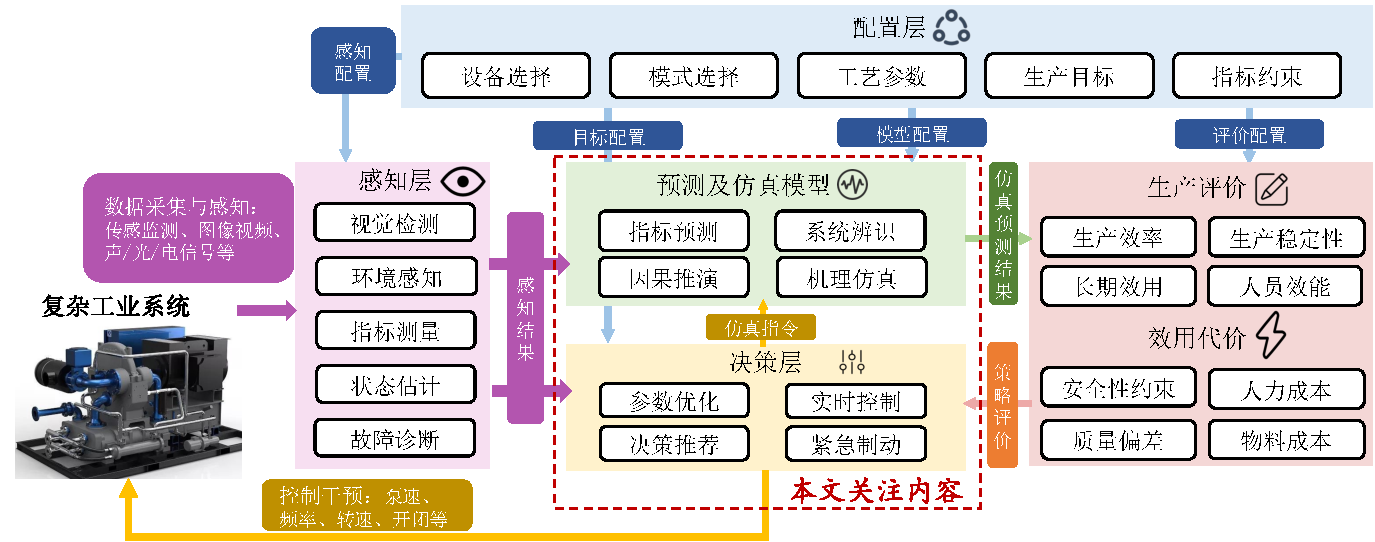
\includegraphics[width=\linewidth]{figures/chapter1/industrial_ai.pdf}
    \caption{面向复杂工业设备感知、建模、评价、决策一体化的通用人工智能实现思路}
    \label{fig:industrial_ai}
\end{figure}

在上述体系架构中,感知层作为人工智能领域近十年来的热门研究方向,相较于其他板块发展较为成熟,如状态分类、参量回归预测、目标检测、语义分割等技术,只要训练数据充足,很多场景下可以作为整体人工智能方案中可依赖的模块。
生产评价模块的构建往往依赖于人的经验以及外部限制,比如误差代价、安全约束、运行成本等,需要根据生产目标、系统特性以及外部环境进行针对性设计。
% 从机器智能以及数据驱动可以一定程度上地帮助决策人员发现一些潜在的优化目标以及更长期的效用评价,但能够发挥的作用相对有限。
% 预测与仿真以及智能决策优化作为实现复杂工业系统控制优化的基础,是实现感知、决策、评价一体化闭环智能的关键环节。
相较于其他模块而言,现有的预测建模以及决策优化方法在解决复杂系统问题时存在一定局限,严重制约了的工业通用人工智能技术的发展。
% 相较于其他板块而言,现有的预测建模以及决策优化方法在模型适用性、非确定性及非线性表示、长时延关系建模等方面存在一定局限,难以适用于特性迥异的复杂工业系统,严重制约了的工业人工智能技术的发展。
相较于其他模块而言,现有的预测建模以及决策优化方法在理论体系以及技术方案方面尚不完善,制约了工业人工智能技术的发展。

% 如何建模复杂系统的运行过程并认知系统的内在机理,是实现系统分析优化的基础。
想要实现复杂工业动态系统的建模,并实现系统的决策优化,其本质在于对系统中目标变量的演化机理以及受其他协变量的影响因果关系进行建模,并基于此实现可控变量的逆向优化。
由于在工业环境下,复杂系统的运行过程存在非线性、高扰动、强耦合等复杂特性,从物理、化学、动力学角度建模系统动态过程的传统分析方法不再适用。
伴随着工业监测技术的不断完善以及生产自动化、信息化水平的不断提升,各种大型设备上安装了用于实时监测生产数据的传感器。低廉的数据获取成本以及理论建模的局限性使得数据驱动方法成为建模复杂工业系统过程的主流方案。

最早追溯到1950年,为了进行控制系统设计,文献\cite{zadeh1956identification}首次提出了系统识别的概念用来建模动态系统。
其核心目标是寻找一个与系统“相符”的模型,使得模型预测的输出尽量接近给定真实的系统输出。
以数据为核心驱动力的传统系统识别方法已经发展为一个非常完善且成熟的研究领域。
\cite{le2013system,gevers2006personal,ljung2008perspectives,ljung2011four,Ljung2020}。
伴随着人工智能技术以及机器学习技术的飞速发展,传统控制系统建模与优化领域也迎来了新的发展浪潮。
动态系统建模作为一项被前人深入研究数十载的“经典问题”,逐渐朝着观测更高维、动态更复杂的方向演化。

在《关于发布未来工业互联网基础理论与关键技术重大研究计划2021年度项目指南的通告》中指出,“实现动态扰动下系统分布式资源调控、数据驱动的系统建模、质量预测与控制以及全流程重构的多目标优化,结合航空航天$\cdots\cdots$。”足以说明数据驱动系统建模技术在现代工业智能化发展路线中占据着举足轻重的地位。

AI界当代最著名巨擘之一、Meta的AI实验室灵魂人物Yann LeCun,长期致力于让机器对世界的运转理念有基础了解。在其设计的通用人工智能(Artificial General Intelligence,AGI)架构体系中,设计了配置器、短期记忆模块、感知器、决策器、世界模型、评价模型,其中世界模型放在了与感知器和决策器同等重要的位置上。理想的世界模型能够像拥有“常识”的人类一样,预见给定行为后将产生后果,并辅助智能体决策。
本文探究的动态系统建模问题可以认为是世界模型在低维控制、低维观测限定下的特例。
图\ref{fig:industrial_ai}中定义的单个复杂控制系统的观测、感知、建模预测、决策闭环可以视为一个封闭的“小世界”,本质上与LeCun提出的通用人工智能研究范式极其相似。

从机器学习的视角来看,系统建模本质上是一种有监督学习问题\cite{jordan1992forward}。
对于动态模型,假定其系统状态表示为$s_t$,系统输入为$a_t$,给定批量的状态转移数据,我们可以学习前向模型$\left(s_t, a_t\right) \rightarrow s_{t+1}$,即给定当前状态和动作,预测下一时刻状态。
% 对于所有的基于模型的强化学习,均需要关注于前向模型的构建。
由于现实生活中大部分的客观物理系统具有连续动作空间以及高维观测空间,依赖于表格存储形式的前向模型表示方法难以适用。
函数近似也因此成为当前复杂动态系统建模问题的主流方法。如线性回归\cite{silver2008sample},动态贝叶斯网络、随机森林、最近邻搜索、神经网络\cite{werbos1989neural}。
近十年来,人工智能领域发展迅猛,深度神经网络以其极强的特征提取与非线性表示能力成为解决高维、大数据、多模态机器学习问题的常用解决方案。
基于深度网络模型的复杂系统建模方法逐渐受到大家的关注,
利用神经网路的前向传播过程模拟系统的动态过程\cite{temeng1995model, tan1996nonlinear}。
相比于其他方法,神经网络能够很好地扩展至高维输入输出空间以及非线性系统。
% 特别地,循环神经网络(Recurrent neural network, RNN)因为存在隐状态,可以更好地处理长期预测问题并对系统进行建模\cite{delgado1995dynamic, zamarreno1998state}。
本论文的讨论内容也限定在基于深度学习的系统建模方法中,具体研究面向不同类型动态系统的深度网络设计以及学习方法。

% \subsection{微分方程网络在复杂系统建模中的应用}

依托于数字计算机技术的应用普及,以及近年来机器学习、强化学习\cite{sutton2018reinforcement}、深度学习\cite{lecun2015deep}\cite{duan2016}、时间序列分析等技术\cite{shumway2000time}的快速发展,
离散时间(Discrete-time, DT)角度的动态建模研究方向涌现出了诸多成果,领域发展相对较为成熟,其原因与数字计算机将信息离散化的思想密不可分。
相较于离散时间系统,连续时间(Continuous-time, CT)系统作为最早的系统辨识研究范式,近年来其相关理论体系研究较为滞后。在当今数据驱动与深度学习盛行的时代背景下,尚未与主流技术形成深度融合。但是对比离散时间系统建模方法,从连续时间域角度进行系统建模的思想在\textbf{与物理属性的兼容性、引入先验知识的难易度、处理非均匀采样数据、变化采样间隔、计算效率与精度的可调节性、刚性系统建模}等方面具有天然的优势,而上述特性或问题在复杂工业系统中尤为常见。
因此,如何让深度学习等先进的人工智能技术充分赋能传统的连续时间系统辨识及控制决策理论,是推进传统控制领域发展,加速人工智能技术实现产业应用的有效路径。
% 因此,最早的系统辨识方法研究也大多是围绕连续时间系统展开的。

% 神经网络近似能力的通用性可以作为建模非线性系统的一种手段\cite{funahashi1993approximation},进而拟合函数$f$。

% \subsection{基于编解码结构的系统预测}
% 当系统具有较大时延,即高时滞特性下,模型需要考虑历史数据对未来系统变化的影响。Felipe 等\cite{demeester2020system}利用带有Attention组件的Encoder-Decoder模型对一种名为膏体浓密机系统进行建模识别,Yuan等\cite{Yuan2020}采用一种更复杂的名为双注意力循环神经网络(Dual Attention Recurrent Neural Network, DARNN)的RNN网络对工业系统进行建模,两种方法都考虑了系统变量之间的长期依赖性,利用循环神经网络加Attention机制的强大编码能力,对历史数据、不同维度数据进行信息编码,来辅助输出量的预测,并且利用预测误差对编码器部分进行训练调整。然而两种方法都是针对离散时间系统设计的,不适用于连续时间系统建模问题。
% \section{深度微分方程网络}
% \subsection{深度微分方程网络总描述}
% \subsection{微分方程网络概述}
发表自神经信息处理会议2018(Neural Information Processing,NIPS 2018)的一篇开创性文章\cite{chen2018neural}提出了一种常微分方程神经网络,其采用神经网络参数化微分方程的向量域\cite{kidger2021},
成功搭建了连续时间微分方程与深度学习技术之间的桥梁。
在其基础上,神经受控微分方程网络\cite{kidger2020neural}、神经随机微分方程网络\cite{li2020scalable}、神经偏微分方程网络
\cite{li2020fourier}等其他神经微分方程(Neural Differential Equations, NDEs)被相继提出。
神经微分方程网络(Neural Differential Equation,NDE)兼具现代机器学习以及传统数学建模方法的优势,包括复杂函数的强拟合能力、便于在模型空间中引入强先验假设、处理非均匀采样数据、训练显存占用小等优点。
一经提出就受到了国内外学者的广泛关注,并应用于时间序列分析、时间点过程分析、动态系统建模、可逆生成模型等领域。
许多流行的神经网络架构,如残差网络、循环神经网络均可以视为神经微分方程的离散化形式。

% 微分方程网络因其在显存空间占用、系统先验引入、非均匀采样序列处理等方面具备的显著优势,
% 一经提出就受到了国内外学者的广泛关注,并应用于时间序列分析、时间点过程分析、动态系统建模、可逆生成模型等领域。
% 许多流行的神经网络架构,如残差网络、循环神经网络均可以视为神经微分方程的离散化形式。

% 在处理时间序列问题方面,相比于RNN等离散时间步下的循环神经网络。ODE-Net天然地适用于建模非均匀采样的时间序列。

% 因此神经微分方,
% % 因此开辟了解决连续时间系统建模问题的新途径。
% % 神经微分方程网络兼具现代机器学习以及传统数学建模方法的优势,包括复杂函数的强拟合能力、便于在模型空间中引入强先验假设、处理非均匀采样数据、训练显存占用小等优点。

对于大部分工业系统,
% 其底层运行机理遵循化学、动力学、热力学等能够用微分方程描述的基本定律,
其底层运行机理所遵循的化学、动力学、热力学定律均可用连续时间微分方程描述,这与微分方程网络的基本特性极其契合。
% 因此利用连续时间网络模型对物理系统进行建模可以更好地匹配客观世界物理规律,且增加模型的可解释性。,
因此NDE成功开辟了解决连续时间域下复杂系统建模问题的新途径。
\textbf{然而在工业领域中,大部分的动态系统机理复杂、特性迥异,基于单一前馈神经网络的神经微分方程无法适用于所有建模任务},需要结合被建模系统的不同特性、训练数据的统计规律、辨识模型的预测需求,设计合理的参数化模型结构,并选用合理的优化目标与训练方法以获得最佳的建模效果。
因此,本文以膏体浓密机、工业制冷系统等复杂工业设备及生产过程为对象,面向长时延非线性、周期多阶段性、随机非确定性等三种复杂特性,提出了三种基于常微分方程网络的系统辨识模型。
并在识别模型的基础上,提出了一种连续时间域下复杂工业系统的在线控制优化方法,并成功应用于工业实践,
成功推进了深度学习技术在真实工业系统建模与决策场景下的落地,
% 该项研究能够有效拓宽连续时间域下深度学习技术及神经微分方程网络的应用边界,
在数据驱动的工业系统建模与优化领域开创新的研究思路。
\section{本文研究的关键问题}
\label{sec:challenge}
% 现有的基于机器学习的系统预测方法多从离散时间域角度描述系统动态过程,并利用数据驱动的方式对离散时间系统参数进行拟合训练。
% 但在复杂工业系统中,上述陈列的系统特性以及问题需求是时常存在的。
% 比如由于不同传感器工作频率不一致会导致数据存在非均匀采样情况,使用离散时间域模型之前需要对数据进行大量的前处理,这会对数据的原始特性造成损坏。

% 连续时间域模型对于复杂动态系统具有天然契合性,深度学习方法在参数化建模与复杂系统表示方面具有较大优势。
% 因此,本论文从二者结合的角度,对基于深度微分方程网络的复杂动态系统预测技术开展研究。
% 利用参数化的深度神经网络模型拟合复杂系统的微分方程,并基于拟合模型实现系统的预测、控制与优化。
神经微分方程网络兼具了深度学习模型的强拟合能力与微分方程的连续时间演化特性,
% 使用连续时间域的深度神经网络模型拟合复杂动态系统,会面临以下研究难点与挑战:
但是使用该模型拟合复杂动态系统时,由于系统存在各类复杂特性,常规网络结构及建模方法会面临以下研究难点与挑战:
\subsection{具有长时延、强非线性的复杂连续时间系统建模问题}
% 随着大数据采集与处理技术的不断进步,很多企业会在复杂工业设备上安装大量传感器以监测工业系统的实时运行过程。
解决复杂系统的控制决策难题,模型预测控制方法首先利用传感器监测工业系统的实时运行数据并训练时序预测模型,然后采用基于预测模型的系统优化及控制策略对可控变量进行优化~\cite{Yuan2020,Member2019,wu2020optimization}。
现有的辨识与预测方法在解决复杂工业系统建模问题时难以解决两方面问题,首先大多数工业系统都有极其复杂的高阶动力学方程,它们不是仿射系统或线性系统,经典的系统假设及参数估计方法无法适用。
另外,对于非马尔科夫系统,当前输出的变化可能受很长一段时间内系统外部输入的影响,直接建模输入输出之间的微分方程难以从数据中捕捉系统的长时延特性。
% 其次,现有的大多数基于深度学习的系统建模及预测方法~\cite{Member2019,Essien2020,9161367,9522017,neu2021systematic}都是基于离散时间域的,忽略了系统的连续时间特性。从模型结构与系统本体的一致性角度来看,忽视系统本身具备的物理先验特性会增大模型的假设空间进而导致增加拟合难度,在数据集有限的情况的下,限制了模型精度。
% 最后,基于数据驱动的自回归系统辨识模型受制于预测过程累积误差的存在,难以同时处理系统短期预测和长期预测。
最后,原始的常微分方程网络对导函数不断进行积分,其模型本质类似于在离散时间序列预测问题中学习序列的差分,在短期预测时模型精度较好。但在长序列开环预测时,对导数持续积分会造成极大的累积误差。

因此,本文围绕连续时间视角下的深度系统辨识模型进行研究,预期解决长时延、非线性复杂动态系统的长短期开环预测问题。

\subsection{具有周期多阶性的连续时间跳变系统建模问题}
跳变系统是一种在多个子阶段之间随机切换的非线性系统,每阶段下的系统动态方程彼此不同,在每个阶段内的滞留时间会同时受到内部和外部因素的影响~\cite{WANG2022111790}。
为了从给定数据中学习连续时间跳变系统,以往的研究一般限定了系统的先验结构,采用EM算法(Expectation-Maximization Algorithm)\cite{balenzuela2022parameter}、序列蒙特卡罗(SMC)\cite{6859280}和变分推理\cite{opper2007variational}等方法估计系统参数。
上述方法通常依赖于对系统结构和阶段滞留时间分布的先验认识,这对于部分复杂“黑盒”跳变系统来说是极其困难的。
% 这需要大量的领域知识支撑。
% 但是,系统结构和参数往往是未知的,阶段转换时间也并非服从理想的指数分布。
% 但是对于部分复杂的“黑盒”跳变系统,系统结构和参数均是未知的,阶段转换时间也并非服从理想的指数分布。
% 跳变系统建模的另一个困难是数据集中可能同时涵盖多个具有不同动态特性的多个子过程,不同子阶段之间的转换规则很难识别。
以往的一些研究采用基于深度学习的自适应性模型识别此类具有多个子过程的复杂时变“黑盒”系统。
深度状态空间模型~\cite{Deep_state_space_model}利用参数动态变化的线性状态空间模型建模系统输出,并引入循环神经网络(RNN)建模参数的演化过程。
其他研究如Embed to Control(E2C)~\cite{Watter2015}和卡尔曼变分自编码器(KVAE)~\cite{Fraccaro2017}采用多个时不变的线性状态空间模型建模系统在隐空间中的不同动态,并推断出随时间变化的权重$\alpha(t)$以分配每个线性状态空间模型的权重。
上述用于建模时变动态系统的混合模型假定目标系统由多个“黑盒”子系统按权重混合而成。
而在某些情况下,对于一些自切换的跳变系统,系统在某一时刻的所处阶段是唯一的且阶段转移边界是明确的。
目前尚无研究将系统阶段转移的先验知识引入到辨识模型的设计中,以预测跳变系统中的阶段自切换。  
另外,对于带有多输出项的工业系统,其输出空间同时存在稳定和非稳定过程\cite{nason2006stationary}。
目前,对于现有的未经过特定设计的预测模型难以解决此类带有混合时序特性的系统学习任务。

因此,本文将着重研究具有多输出量的连续时间跳变系统建模方法,针对多阶段之间周期性转换以及稳定、非稳定输出共存的跳变系统,提出基于常微分方程网络的系统建模解决方案,依赖已知的系统先验特性提高模型的辨识精度。

\subsection{具有随机性、非确定性的复杂连续时间系统建模问题}
现存的连续时间系统辨识及动态系统建模方法,如Time-Aware RNN\cite{Demeester2019}、SNODE\cite{Quaglino2019} 仅在确定性状态空间对模型进行表示。
由于确定性模型没有引入任何随机性成分,不便于实现蒙特卡洛随机采样,这使得某些基于随机采样预测的控制规划方法,如交叉熵(Cross entropy Maximum,CEM)、蒙特卡洛树搜索(Monte Carlo Tree Search,MCTS)难以与此类系统建模方法配合使用。
另外,确定性模型无法适用于建模带有随机性的模型。当被辨识系统的状态转移过程本身具备较强的随机性时,可以近似认为状态之间的转移过程服从某种复杂的分布,理想的辩识模型应该能够直接对该分布进行建模,如离散时间域下的循环状态空间模型\cite{Hafner2019}(Recurrent State Space Model, RSSM)。
最后,确定性模型无法对系统当前状态的非确定性进行度量与表示。
因为在现实世界中,尽管很多系统的转移过程本身是确定的,但由于其观测空间的不完备性,从可观测的输入输出数据中无法准确推理系统的完整状态,从结果来看这种部分可观测性近似等价于随机性。

现有连续时间域的系统辨识方法仅能在隐空间中隐式地对系统的非确定性进行编码,而无法对其显示地量化与评估,制约了模型的可解释性与拟合能力。
% 在建模随机非确定系统方面,深度时序生成模型~\cite{Fraccaro2016,Chung2015,Karl2017}将标准的变分自编码机(Variational Auto-encoders,VAEs)~\cite{kingma2013auto}扩展到序列情况下,
% 通过在隐空间引入随机隐变量学习序列的随机性,然而这些方法均是离散时间域模型。

因此本文着重研究存在随机性、非确定性的复杂系统连续时间域系统建模方法,使辨识模型能够对系统的随机特性进行拟合,并在给定观测数据下评估系统的非确定性。

\subsection{复杂工业系统的控制策略构建与自适应优化问题}
大部分复杂工业生产过程往往伴随着较强的非线性、非确定性、高时滞性,因此难以建立准确的数学模型近似其运转机理, 导致传统的控制优化方法无法适用于此类复杂工业设备。
% 为了解决复杂工业设备难以建立准确的数学模型,导致传统的控制优化方法无法适用于此类复杂工业设备。
目前业界对基于强化学习理论的最优控制技术\cite{Sutton2018}\cite{F.L.LewisD.Vrabie2012}寄予厚望,希望能够以免模型、数据驱动的方式实现复杂工业系统的自适应优化控制。
Wei等\cite{Wei2014}将煤炭气化过程的最优追踪控制转化为双人零和最优控制问题,并采用包含控制网络、模型网络、评价网络的迭代自适应动态规划方法求解最优控制律,同时给出了收敛稳定性的分析。
Jiang等\cite{Jiang2018}利用穿插学习策略迭代(Interleaved Learning
Policy Iteration, ILPL)并同样采用三网结构实现了对浮选过程操作指标优化的控制,获得了比传统值函数迭代(Value iteration, VI)、策略迭代(Policy iteration, PI)算法更佳的控制效果。
然而,考虑到工业过程试错成本高,大部分强化学习算法随机设定策略模型的参数,在模型训练初始阶段,难以保证生产过程的安全。
另外,在工业场景下进行设备在线控制对算法的实时性要求较高。为了保证控制模型的控制效果,需要采用实时生成的数据对网络进行训练,使得训练过程产生较大的时间开销,模型更新与推理的实时性难以保证。
最后,受限于无模型强化学习存在高采样成本与低场景泛化能力等缺陷,无模型强化学习算法在真实的工业实践中难以部署应用。

因此本文研究连续时间域下基于模型的复杂工业系统优化控制策略,充分利用系统运行时的非均匀采样离线数据构建预测模型,并在辨识模型的基础上构建具有在线自学习能力的控制决策模型。
% 能够适应物料性质改变、设备老化等被控系统不断变化的情况。

\section{本文的研究内容}
% 针对上述问题与挑战, 本文以具有连绔时间动态特性的复杂系统作为研究对 象,针对系统存在的非线性、非确定性、多阶段混合、高时延、不同输出量统计特 征不一致等特性, 将连绔时间域模型的灵活性与深度神经网络的强大表示能力相
% 针对第\ref{sec:challenge}节提出的系统存在的高时延、非线性、随机非确定性、周期多阶段性、不同输出量统计特征不一致等复杂特性特性,
针对第\ref{sec:challenge}节提出的复杂工业系统难以建模预测及优化控制的问题。
% 本文以具有连时间动态特性的复杂系统作为研究对 象,针对系统存在的非线性、非确定性、多阶段混合、高时延、不同输出量统计特 征不一致等特性, 将连绔时间域模型的
本文以具有连续时间动态特性的复杂系统作为研究对象,
针对系统存在的非线性、非确定性、多阶段混合、高时延、不同输出量统计特征不一致等特性,
依托于连续时间域模型的灵活性与深度神经网络的强大表示能力,研究基于连续时间深度时序网络的系统建模方法。
并在识别模型的基础上,研究基于有模型强化学习理论的在线优化控制方法,并应用于工业实践。
% 针对复杂系统存在的非线性、非确定性、多阶段混合、高时延、不同输出量统计特征不一致等特性,本文开展了如下几方面的研究:
图\ref{fig:study_goal}展示了本文研究内容、研究目标以及相关科学问题的对应关系。
\begin{figure}[h]
    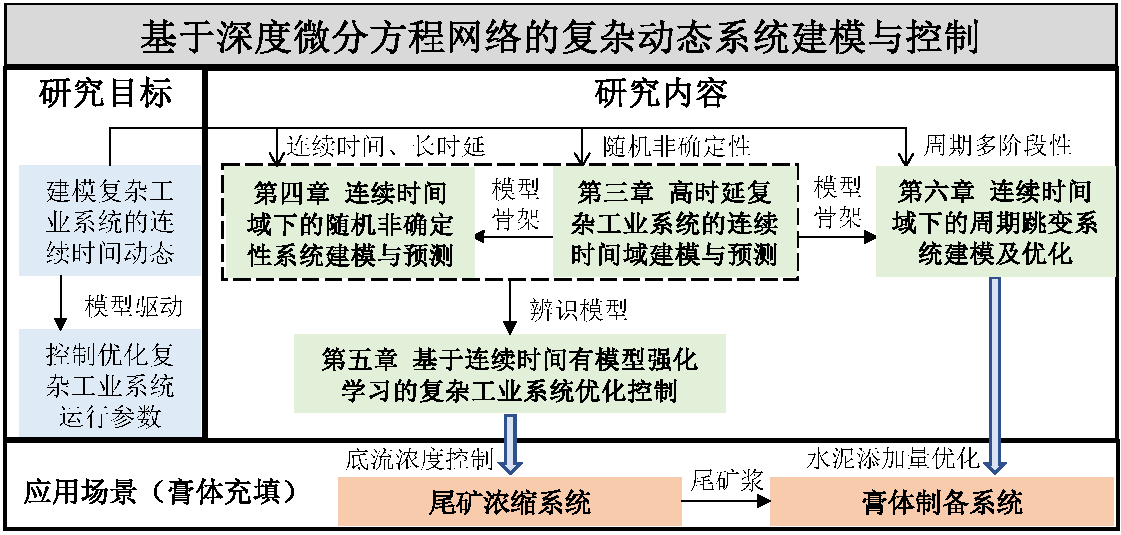
\includegraphics[width=\linewidth]{figures/chapter1/study_goal.pdf}
    \caption{本文研究内容、研究目标及关键问题的对应关系}
    \label{fig:study_goal}
\end{figure}
接下来,将给出每一项研究内容的研究思路和简要介绍。

\subsection{基于可微ODE-Net的高时延复杂工业系统预测}
第一项研究内容基于可微ODE-Net的高时延复杂工业系统预测,重点讨论了连续时间视角下,非线性、高时延系统的系统建模问题。
大部分复杂工业系统反馈延迟长,现有辨识方法难以拟合长距离的依赖关系,如果从状态空间模型的角度将系统状态和输入记忆进行压缩,会对待学习过程引入了极强的复杂性与非线性。
另外基于数据驱动的自回归系统辨识模型受制于预测过程累积误差的存在,难以同时处理系统短期预测和长期预测问题。
因此需要从探索\textbf{参数化微分方程网络对于客观世界连续时间过程的可拟合性}这一科学问题出发,研究深度学习网络与连续时间过程相结合的系统建模方法。

本文的第一个研究内容为了克服动态系统存在的非线性、非仿射的高复杂性。研究了基于深度学习的复杂工业系统建模方法,同时为了契合生产设备运转本质为连续时间过程的特性,提出以ODE-net作为模型骨架结构,从连续时间域角度拟合复杂工业系统的动态过程。
针对系统输入输出之间长时延依赖关系难以建模的问题,研究了基于序列自编码器模型的输入输出长距离信息连接通道构建方法。
针对深度序列模型受制于累积预测误差,难以有效进行长期预测的问题,基于时间序列稳定性理论,分析了普通常微分方程网络在长期预测中的非稳定特性,并提出两种分别适用于短期预测和长期预测任务的导数模块定义方法。同时,针对ODENet网络训练需要连续控制输入信号的问题,研究了面向训练过程的离散输入点并行插值方法。最后,提出了一套由序列编码器、状态解码器和导数模块组成的深度连续时间(Continuous Time, CT)系统辨识网络模型,能够以端到端的方式学习工业系统输出的自回归变化过程和输入对输出的非线性影响。
通过消融实验探究了编码器输入序列长度、微分方程求解器选择对于预测精度的影响。最后,通过某真实铜矿场中膏体浓密机的运行数据验证了本文提出方法在解决高时延、非线性复杂系统长短期预测问题的有效性。


% 针对复杂工业系统本质上为连续时间演化过程,且存在非线性、长时延等特性,本文提出以ODE-net作为模型骨架结构,从连续时间域角度拟合复杂工业系统的动态过程。


\subsection{基于自跳跃-常微分方程网络的连续时间周期性跳变系统建模}


% 2) 基于有限状态机-常微分方程网络的周期性多阶段复杂系统建模 \\
第二项研究内容基于自跳跃-常微分方程网络的连续时间周期性跳变系统建模重点讨论了连续时间视角下周期跳变系统建模问题。
工业场景中,系统在不同阶段下的动态特性彼此迥异,且各阶段出现的持续时间、状态转换的触发条件会同时受到内部、外部多种混杂因素共同影响,其影响机理复杂,可能超出领域知识的可解释范畴。
因此,如果想要结合参数化深度模型对具有跳变特性的多阶段系统以端对端的方式进行数据驱动建模,需要从探索\textbf{跳变系统阶段滞留时间及转移机制的可学习性}这一科学问题出发,
研究符合跳变系统先验特性的且具有阶段自识别、自转移能力的多阶段深度辨识方法。

具体地,该研究内容针对周期多阶段系统在不同阶段下动态特性彼此迥异,难以统一建模的问题,
研究了传递式多ODE-Net集成结构,以独立建模系统在不同阶段下的动态特性,并支持开环预测阶段转换处隐空间的状态衔接。
针对阶段持续时间难以预测、转换条件和位置难以识别的问题,
提出了跳变系统辨识问题中的自跳跃(Autonomous jump)概念,
并在多ODE-Net集成架构的基础上,研究了基于阶段持续时间预测网络的阶段自转移方法。
除此之外,针对工业系统的多输出项可能同时存在稳定特性和非稳定特性的情况,研究了不同类别输出项的解藕建模方法,并提出了稳定ODE与非稳定ODE相结合的分层常微分方程网络单元。最后,通过某真实工业制冷系统的的运行数据验证了本文提出方法在解决多输出周期跳变系统建模问题的有效性。


\subsection{基于深度常微分方程-马尔可夫模型的随机非确定性系统建模}
% 3) 基于常微分方程-循环状态空间模型的随机系统建模 \\

第三项研究内容“基于深度常微分方程-马尔可夫模型的随机非确定性系统建模”重点讨论了连续时间视角下,随机非确定性复杂系统建模的诸多问题。
现实世界中的复杂系统往往具备典型的随机性(Uncertainy)和非确定性(stochasticity),确定性系统辨识模型只能以最小化期望误差的方式拟合系统随机演化函数在某分布下的期望,不仅不便于实现系统的随机采样预测,且无法对可观测数据呈现出的非确定性和随机性给出表示与度量。因此,想要在辨识模型中引入对于系统随机非确定性的感知与描述能力,并给出概率域下的识别及预测结果,需要从“\textbf{部分可观测马尔可夫决策系统的随机性、非确定性产生机理}”这一科学问题出发,研究贝叶斯视角下隐空间状态的时序生成过程及逆向推理方法。

具体地,针对随机非确定性连续时间系统难以表征、建模的问题,
研究向确定性微分方程系统演化中添加随机转移路径的有效途径,
进而提出深度常微分方程与马尔可夫模型相结合的随机非确定性系统建模方法,并结合时序变分推断理论给出训练模型所需要优化的证据下界。
同时,针对训练阶段下原始时序变分推理算法无法实现沿时间反向传播(Backpropagation through time, bptt)难以保证多步预测精度的问题,
研究了基于采样状态重用的高效隐空间超调技术,进而在不增加训练时间开销的情况下显著提升模型的开环预测精度。
最后,针对训练阶段批数据中不同常微分方程积分区间不一致导致难以并行化训练的问题,研究了基于重参数变换的批常微分方程并行求解技术,成功实现了不同积分区间下的高效并行训练。
最后,通过三个输入输出系统数据集验证了本文提出方法在解决随机非确定性系统建模及多步开环预测问题中的有效性。
\subsection{基于连续时间深度强化学习的复杂工业系统优化与控制}
第四项研究内容“基于连续时间深度强化学习的复杂工业系统优化与控制”重点讨论了连续时间视角下,基于数据驱动的复杂非线性工业系统的优化控制方法。
大部分复杂工业系统的运行过程具有不完全观测、非线性、多变量、高时滞等特点,
想要建立准确的数学模型描述其运转机理是极其困难的,因此基于模型的传统最优控制理论及方法难以适用。系统运行过程产生的历史数据为无模型数据驱动优化控制提供了可行的思路。
% 想要充分利用离线数据构建近似的系统模型并衍生形成可靠的控制策略,
% 需要从“\textbf{数据驱动建模对于免模型强化学习的可改善性}”这一科学问题出发,研究基于辨识模型指导的复杂工业系统强化学习控制方法。
想要充分利用离线数据构建近似的系统模型并衍生形成可靠的控制策略,
需要以动态系统辨识为基础,研究基于辨识模型指导的复杂工业系统强化学习控制方法。

具体地,针对非线性、高时滞复杂工业系统控制优化难的问题,研究了基于数据驱动的有模型自适应动态规划控制方法,定义了系统的状态空间、动作空间、效用函数、状态转移函数等内容,并提出了离线系统建模与在线强化学习相结合的原始控制器构建及生产环境在线学习策略,通过利用离线采集数据以及在线监测数据有效解决了复杂工业系统控制优化难的问题。
同时针对在线环境下策略网络增量训练开销大的,在线学习与控制难以满足实时性的问题,研究了基于自适应评价值迭代的控制动作求解算法,通过在模型架构中去掉策略网络有效减少了在线学习的计算开销。
另外,针对评价模块参数收敛慢、难以准确给出策略优化方向的问题,研究了基于短期经验回放的评价网络训练技术,有效提高了模型对于局部评价值梯度变化的敏感性及预测准确性。
最后,本文选用一种典型的复杂工业系统——尾矿浓缩机,利用其仿真模型验证了本文提出的自适应控制算法在控制精度、时间消耗方面的优势。
同时将该控制算法应用于某真实矿山的深锥浓密机底流浓度控制场景中,相比于原始的规则控制算法,大幅度提高了出料浓度的追踪控制效果及稳定性。

\section{论文的章节安排}

本文针对连续时间域下的复杂动态系统建模及控制中的关键技术开展研究,全文共分为七章,各章主要研究内容及之间的关系如图\ref{fig:structure}所示:
\begin{figure}
    \centering
    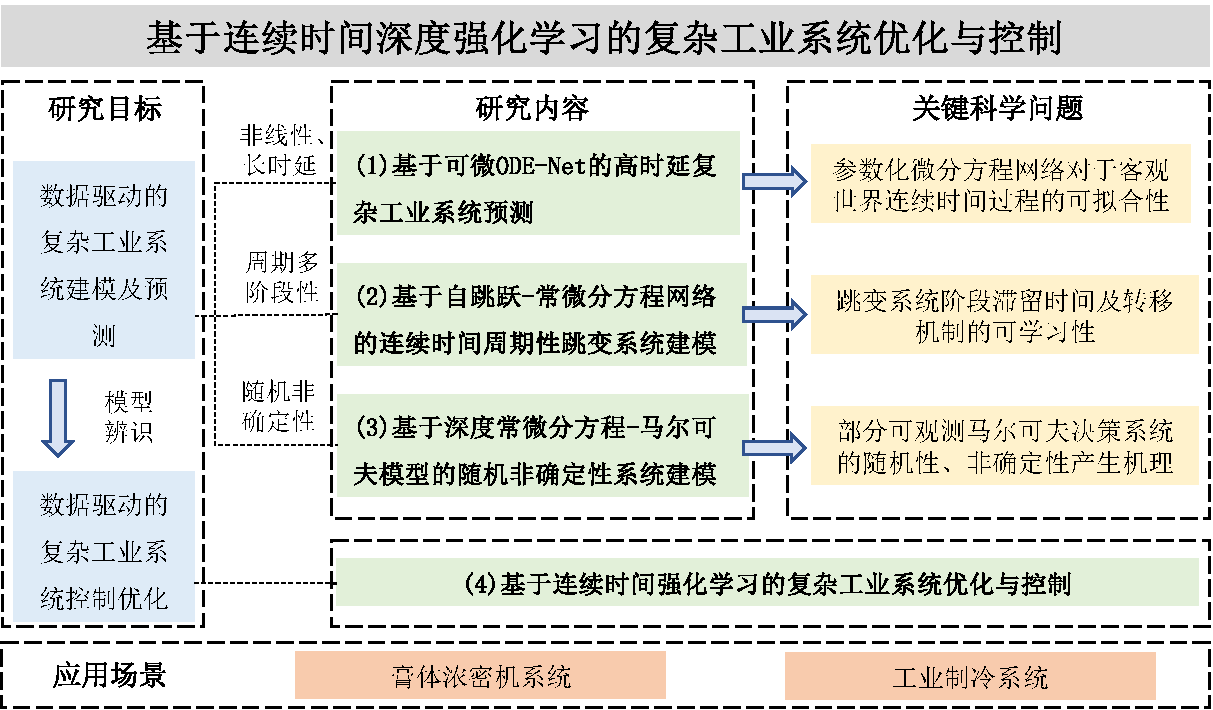
\includegraphics[width=0.95\linewidth]{figures/chapter1/structure.pdf}
    \caption{论文组织结构}
    \label{fig:structure}
\end{figure}

第一章介绍本文工作的研究背景及意义,提出了基于数据驱动的复杂系统建模方法所面临的难点与挑战,并总结了本文的主要研究内容与创新点。
第二章介绍了国内外关于数据驱动的动态系统建模的研究现状。
第三章到第六章是本文的主体部分,详细介绍了本文的所有研究内容。

% 第二章对于复杂系统的预测方法及深度微分方程网络的原理及技术进行介绍。

第三章研究了基于可微ODE-Net的高时延工业多输入输出系统预测,首先介绍了复杂输入输出系统预测问题的形式化表述并给出基于状态空间模型的表示方法。
进一步地,介绍了本文提出的基于ODE-Net的连续时间输入输出系统预测模型,并分别介绍其序列编码器、导数模块以及状态解码器三大组成模块,同时给出了基于伴随状态的模型训练方法。
另外,该章针对短期预测和长期预测两种预测场景,给出了两种导数模块定义方法。
并提供了用于连续化系统输入序列的并行插值方法。
最后,该章介绍了将上述模型应用于膏体浓密机系统预测问题的实验结果。并从微分方程求解器的选择、序列编码器输入的长度设定等多个角度进行了消融实验。

% 第三章研究了基于有限状态机-常微分方程网络的周期性多阶段复杂系统预测建模技术,分别介绍了周期性多阶段系统的形式化定义,H-ODEnet结构设计,DFA-ODEnets模型结构设计、基于DFA-ODEnets的编码器解码器结构设计。
第四章研究了基于自跳跃常微分方程网络的连续时间跳变系统建模
首先给出了连续时间跳变系统的变量符号定义以及系统预测问题的形式化描述。
其次,介绍了本文提出的分层常微分方程网络的定义及结
构,及如何将其用于学习同时带有稳定和非稳定时间序列输出的动态过程。
在此,提出了用于建模连续时间周期跳变系统的自跳跃常微分方程模型,并详细阐述了其状态转移方程、持续时间预测器等关键模块结构的定义。
进一步地,给出了基于该模型的编码器解码器框架及其训练方法。
最后,实验环节介绍了如何将上述框架应用于模拟某实际工业制冷系统,预测给定热负载下的制冷功耗以及出气口温度变化,
同时基于预测仿真结果,对制冷系统的起停温度设定值进行优化。

第五章研究了基于深度常微分方程-马尔可夫模型的随机非确定性系统建模,首先给出了非均匀采样下随机系统的形式化描述及符号变量定义。
技术部分首先介绍了本文提出的常微分方程-循环状态空间模型,包括其时序受控生成过程及隐变量的后验推理过程。
并基于时序变分推断方法给出了用于训练模型的单步证据下界。
进一步地,为了改善模型的多步预测性能,在单步下界的基础上提出了基于隐空间超调的多步变分下界。
最后,提出了非均匀采样间隔下的批量常微分方程并行化求解方法以加速训练。
实验环节采用两个共有数据集、一个私有数据集对常微分方程-循环状态空间模型以及多个基线模型在非均匀采样设定下的随机采样系统建模问题的有效性进行评估,并对多步预测性能
实验环节采用两个共有数据集、一个私有数据集对常微分方程-循环状态空间模型以及多个基线模型进行对比评估,
同时验证了隐空间超调技术对于多步预测的改善效果以及非均匀间隔批常微分方程并行求解算法的有效性。


第六章研究了基于连续时间深度强化学习的复杂工业系统优化与控制,
首先给出了基于连续时间强化学习的非线性系统控制过程的符号变量定义、形式化描述。
技术部分主要介绍了本文提出的启发式评价网络值迭代控制算法,首先描述了如何利用常微分方程网络学习被控系统的近似参数化模型,然后基于积分强化学习理论给出折扣积分奖赏的定义及表示形式,并介绍如何利用评价网络对策略评价值进行近似。进一步地,介绍了基于随机梯度下降的动作生成策略,最后描述了评价网络训练时,为了提升局部评价值梯度变化拟合结果的准确度,所采用的短期经验回放技术。
% 最后,本文选用一种典型的复杂工业系统——尾矿浓缩机,利用其仿真模型验证了本文提出的自适应控制算法在控制精度、时间消耗方面的优势。
% 同时将该控制算法应用于某真实矿山的深锥浓密机底流浓度控制场景中,相比于原始的规则控制算法,大幅度提高了出料浓度的追踪控制效果及稳定性。
实验环节评估了本文提出控制算法在浓密机仿真模型及某矿山真实深锥浓密机底流浓度控制问题中的有效性。


第七章对本文工作主要研究贡献和创新点进行了总结,
最后面向对基于数据驱动的动态模型构建乃至世界模型构建问题,给出了几点关于向模型中有效引入先验知识的研究展望。
